%%%%%%%%%%%%%%%%%%%%%%%%%%%%% Define Article %%%%%%%%%%%%%%%%%%%%%%%%%%%%%%%%%%
\documentclass[a4paper,11pt]{article}
%%%%%%%%%%%%%%%%%%%%%%%%%%%%%%%%%%%%%%%%%%%%%%%%%%%%%%%%%%%%%%%%%%%%%%%%%%%%%%%
\usepackage[utf8]{inputenc}
\usepackage[T1]{fontenc}
\usepackage{helvet}
\renewcommand{\familydefault}{\sfdefault}
%%%%%%%%%%%%%%%%%%%%%%%%%%%%% Using Packages %%%%%%%%%%%%%%%%%%%%%%%%%%%%%%%%%%
\usepackage{graphicx}
\usepackage{amssymb}
\usepackage{amsmath}
\usepackage{amsthm}
\usepackage{empheq}
\usepackage{mdframed}
\usepackage{booktabs}
\usepackage{lipsum}
\usepackage{graphicx}
\usepackage{color}
\usepackage{psfrag}
\usepackage{pgfplots}
\usepackage{bm}
%%%%%%%%%%%%%%%%%%%%%%%%%%%%%%%%%%%%%%%%%%%%%%%%%%%%%%%%%%%%%%%%%%%%%%%%%%%%%%%
\usepackage[colorlinks=true]{hyperref}
\hypersetup{
    colorlinks=true,
    linkcolor=blue!50!black,
    filecolor=blue!50!black,
    citecolor = green!50!black,      
    urlcolor=cyan,
}
\usepackage{fancyhdr}
\usepackage{amsmath}
\usepackage{amsthm}
\usepackage{empheq}
\usepackage{bm}
\usepackage{tikz}
\usepackage{subcaption}
\usepackage{multicol}
\usepackage{authblk}
\usepackage[left=3cm,right=3cm,top=2cm,bottom=2cm]{geometry}
\newcommand{\avg}[1]{\left<#1\right>}
\newcommand{\avgcond}[1]{\overline{#1}}
\newcommand{\oneavg}[1]{\avgcond{#1}^1}


% Other Settings
%%%%%%%%%%%%%%%%%%%%%%%%%% Page Setting %%%%%%%%%%%%%%%%%%%%%%%%%%%%%%%%%%%%%%%

\usepackage{natbib}
\bibliographystyle{plain}
\usepackage{enumitem}
\setlist{nolistsep}
%%%%%%%%%%%%%%%%%%%%%%%%%% Define some useful colors %%%%%%%%%%%%%%%%%%%%%%%%%%
\definecolor{ocre}{RGB}{243,102,25}
\definecolor{mygray}{RGB}{243,243,244}
\definecolor{deepGreen}{RGB}{26,111,0}
\definecolor{shallowGreen}{RGB}{235,255,255}
\definecolor{deepBlue}{RGB}{61,124,222}
\definecolor{shallowBlue}{RGB}{235,249,255}
%%%%%%%%%%%%%%%%%%%%%%%%%%%%%%%%%%%%%%%%%%%%%%%%%%%%%%%%%%%%%%%%%%%%%%%%%%%%%%%

%%%%%%%%%%%%%%%%%%%%%%%%%% Define an orangebox command %%%%%%%%%%%%%%%%%%%%%%%%
\newcommand\orangebox[1]{\fcolorbox{ocre}{mygray}{\hspace{1em}#1\hspace{1em}}}
%%%%%%%%%%%%%%%%%%%%%%%%%%%%%%%%%%%%%%%%%%%%%%%%%%%%%%%%%%%%%%%%%%%%%%%%%%%%%%%

%%%%%%%%%%%%%%%%%%%%%%%%%%%% English Environments %%%%%%%%%%%%%%%%%%%%%%%%%%%%%
\newtheoremstyle{mytheoremstyle}{3pt}{3pt}{\normalfont}{0cm}{\rmfamily\bfseries}{}{1em}{{\color{black}\thmname{#1}~\thmnumber{#2}}\thmnote{\,--\,#3}}
\newtheoremstyle{myproblemstyle}{3pt}{3pt}{\normalfont}{0cm}{\rmfamily\bfseries}{}{1em}{{\color{black}\thmname{#1}~\thmnumber{#2}}\thmnote{\,--\,#3}}
\theoremstyle{mytheoremstyle}
\newmdtheoremenv[linewidth=1pt,backgroundcolor=shallowGreen,linecolor=deepGreen,leftmargin=0pt,innerleftmargin=20pt,innerrightmargin=20pt,]{theorem}{Theorem}[section]
\theoremstyle{mytheoremstyle}
\newmdtheoremenv[linewidth=1pt,backgroundcolor=shallowBlue,linecolor=deepBlue,leftmargin=0pt,innerleftmargin=20pt,innerrightmargin=20pt,]{definition}{Definition}[section]
\theoremstyle{myproblemstyle}
\newmdtheoremenv[linecolor=black,leftmargin=0pt,innerleftmargin=10pt,innerrightmargin=10pt,]{problem}{Problem}[section]
%%%%%%%%%%%%%%%%%%%%%%%%%%%%%%%%%%%%%%%%%%%%%%%%%%%%%%%%%%%%%%%%%%%%%%%%%%%%%%%

%%%%%%%%%%%%%%%%%%%%%%%%%%%%%%%%%%%%%%%%%%%%%%%%%%%%%%%%%%%%%%%%%%%%%%%%%%%%%%%
\fancyhead[L]{
\includegraphics[scale=1]{image/logo.png}}

%%%%%%%%%%%%%%%%%%%%%%%%%%%%%%% Title & Author %%%%%%%%%%%%%%%%%%%%%%%%%%%%%%%%
% \title{{\Large  Toward a generalized hydrodynamic drag law for cylinder particles, Suspensions dynamics of cylindrical particles,} }
\author{\large GAMET Lionel}
\author{\large PIERSON Jean-Lou}
\author{\large GAMET Lionel$^1$, PIERSON Jean-Lou$^2$ and FINTZI Nicolas$^3$}
%%%%%%%%%%%%%%%%%%%%%%%%%%%%%%%%%%%%%%%%%%%%%%%%%%%%%%%%%%%%%%%%%%%%%%%%%%%%%%%
\newcommand{\size}{0.6}
\begin{document}
\begin{flushright}
    FINTZI Nicolas
    
    Fintzi.Nicolas@ifpen.fr
\end{flushright}
\begin{center}
    % \normalsize \hrule height 0.3ex \vspace{0.2ex} \hrule height 0.1ex
    \vspace{10pt}
    {\Large Theoretical calculation of the droplet induced agitation (or pseudoturbulence) of buoyant emulsions in low inertia and dilute regime.
    With Nearest-particle-statistics.}\\
    \vspace{10pt}
    % \normalsize \hrule height 0.1ex \vspace{0.2ex} \hrule height 0.3ex

    \vspace{15pt}
    {\large FINTZI Nicolas$^{1,2}$, PIERSON Jean-Lou$^1$ and POPINET St\'ephane$^1$}
\end{center}
% \maketitle

\begin{flushleft}
$^{1}$\large IFP Energies Nouvelles, Rond-point de l’echangeur de Solaize, 69360 Solaize.

$^{2}$\large Sorbonne Universit\'e, Institut Jean le Rond d'Alembert, 4 place Jussieu, 75252 PARIS CEDEX 05, France.

% Fintzi.Nicolas@ifpen.fr

% Jean-Lou.Pierson@ifpen.fr

% Lionel.Gamet@ifpen.fr

\end{flushleft}
\begin{itemize}
\item Topic : Hydrodynamics of cylindrical particles;
\item Communication preference : Oral presentation;
\item Keywords : hydrodynamics, fixed beds, cylindrical particles, DNS, OpenFOAM;
\item Speaker : FINTZI Nicolas / Fintzi.Nicolas@ifpen.fr
\end{itemize}


\vspace{15pt}

Buoyancy-driven droplet flows are encountered in many chemical engineering processes such as gravity separators and liquid-liquid extractors. 
The usual engineering practice to model such facilities is to use the averaged Navier-Stokes equations. 
These equations require closure laws \citep{jackson1997locally}. 
The present work focus on the velocity fluctuations tensor, also called the \textit{Reynolds stress} tensor. 

Let, $\avg{\ldots}$ denote an ensemble average operator, $\textbf{u}_f^0$ the local fluid velocity and $\chi_f$ the continuous phase indicator function.
Then, $\textbf{u}_f' = \textbf{u}_f^0 - \textbf{u}_f$ is the velocity fluctuation with $\textbf{u}_f =\avg{\chi_f \textbf{u}_f^0} / \phi_f$ the mean continuous phase velocity and $\phi_f = \avg{\chi_f}$ the continuous phase volume fraction. 
With these definitions the \textit{Reynolds stress} tensor of the continuous phase might be written : $\avg{\chi_f \textbf{u}_f' \textbf{u}_f'}$.

This tensor can be decomposed into two contributions : (1) the agitation generated due to the averaged wakes around the particles; (2) all other source of fluctuations such as those generated through particles interactions and the single phase turbulence. 
Formally this is written, 
\begin{equation}
    \avg{\chi_k \textbf{u}'_f\textbf{u}'_f}(\textbf{x})
    = 
    \underbrace{\int_{\mathbb{R}^3}\textbf{u}_f^1\textbf{u}_f^1 P_{f}^1(\textbf{x},\textbf{r}) d\textbf{r} }_\text{(1)}
    \\+\underbrace{\int_{\mathbb{R}^3} \textbf{R} P_{f}^1(\textbf{x},\textbf{r}) d\textbf{r}}_\text{(2)}
    - \phi_f \textbf{u}_f\textbf{u}_f,
    \label{eq1}
\end{equation}
where $P_f^1(\textbf{x},\textbf{r})$ is the probability of finding the fluid phase at \textbf{x} while having a particle center of mass at $\textbf{r}$. 
Additionally, $\textbf{u}_f^1(\textbf{x},\textbf{r},t)$ is the averaged fluid phase velocity conditionally on the presence of a particle center of mass at $\textbf{r}$.
In this sense the first term on the right-hand side is the contribution from the averaged wakes. 
The last term is the contribution from the velocity fluctuation around the conditional velocity $\textbf{u}_f^1$ which is omitted in this study. 

To determine the  $\textbf{u}_f^1(\textbf{x},\textbf{r},t)$ at first order in dispersed phase volume fraction $\phi_d$ one has to solve the conditionally averaged Navier Stokes equation at zero-order volume fraction \cite{hinch1977averaged}.
Therefore, $\textbf{u}_f^1$ can be substituted by the disturbance velocity field of an isolated particle to determine the pseudoturbulence at order zero in volume fraction.
It is in this context that \cite{van1998pseudo} derived a theoritical model for the \textit{Reynolds stress} considering isolated translating bubbles in potential flows, it reads, 
\begin{equation}
    \avg{\chi_k \textbf{u}'_f\textbf{u}'_f}(\textbf{x})
    = \phi \left(\frac{3}{20} U^2\textbf{I} + \frac{1}{20} \textbf{UU} \right)
\end{equation}
where $\textbf{U} = \textbf{u}_d - \textbf{u}_f$ is the drift velocity. 
The integral of \ref{eq1} converged in the case of potential flows since the disturbance velocity field of a translating spherical bubble in potential flow is $\sim \mathcal{O}(r^{-3})$ where $r$ is the distance to the particle center of mass.  
In stokes flows it is well known that the disturbance velocity field of a translating bubble or droplet is $\sim \mathcal{O}(r^{-1})$.
This leads to an infinite \textit{Reynolds stress} according to  \ref{eq1}. 

Eventhrough the limit $\lim_{\phi \to 0} =\avg{\chi_f \textbf{u}_f'\textbf{u}_f'}= \infty$ we might be able to determine the tangent of the \textit{Reynolds stress} at infinity. 
Nevertheless, using \textit{Nearest particle statistics} we are able to by-pass this problem a find the form of the asymmetrical tangent at infinity. 

\begin{figure}[h!]
    \centering
    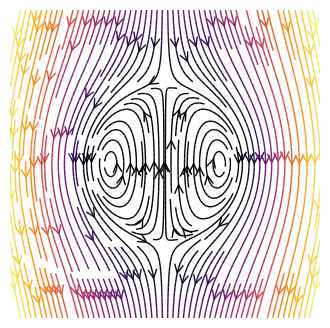
\includegraphics[height=0.3\textwidth]{image/Rising_Stokes.png}
    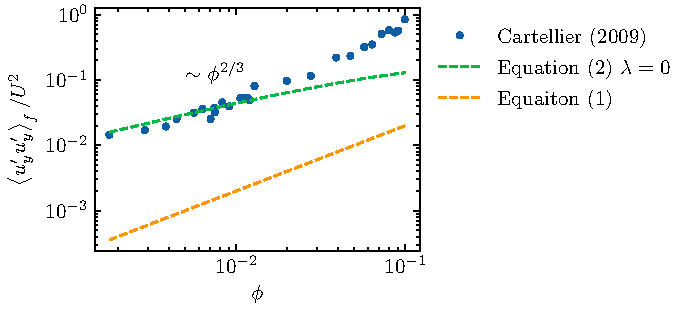
\includegraphics[height=0.3\textwidth]{image/HOMOGENEOUS_NEW/CA/cartellier.pdf}
    \caption{(left) Samples of simulations that will be presented
            (right) Wake around an isolated droplets}
    \label{fig:wake}
\end{figure}


\bibliography{Bib/bib_bulles.bib}
\end{document}
